\graphicspath{{chapters/images/06/}}
\chapter{Assembly}

\section{Introduction}
Assembly is the process of aligning and merging overlapping sequences in longer consensus sequences to reconstruct an original sequence or genome.
No reference database is needed.

    \subsection{Use cases for assembly}
    Assembly is needed to be performed when:

    \begin{multicols}{2}
        \begin{itemize}
            \item Sequencing a genome for the first time.
            \item When the reference genome is not complete or very distant phylogenetically and hence not usable as a reference.
            \item In case of new genes, which cannot be discovered just by mapping.
        \end{itemize}
    \end{multicols}

    This process is rarely needed in human genomics as the human genome is already available.
    By contrast it is particular important in microbial genomics to capture new genes of different strains not present in the reference genome.

    \subsection{General framework for assembly}
    In theory, all assembly algorithms could be based on a basic framework that:

    \begin{multicols}{2}
        \begin{enumerate}
            \item Identifies overlaps between the reads obtained by sequencing.
            \item Connects the reads through those overlaps.
            \item Finds the Hamiltonian paths.
            \item Finds the consensus sequence.
        \end{enumerate}
    \end{multicols}

    In practice this is not always possible, due to many issues that can occur, like:

    \begin{multicols}{2}
        \begin{itemize}
            \item multiple overlapping of the same reads.
                This can be due to high coverage or location in the genomes that match at least partially the reads.
            \item Partial matches.
        \end{itemize}
    \end{multicols}

    One possible solution would be to keep track of all possible matches and then try to reconstruct the sequence.
    One way to represent the possible overlaps between reads is by using a graph in which the nodes represent the reads and the edges represent the connections between the reads that are overlapping in some way.
    Then a mathematical algorithm is needed to find a solution in this very intricate network.
    Many assembly algorithms are available, and they are all based on this idea.
    For this reason, we always end up with multiple copies of genomes, not just one.
    Also, the output is almost never the full genome but pieces of the genome in the form of multiple contigs.
    By default, assembly is done in this way and gives a good representation of the genome, but not complete. Some quality control is also needed, especially to detect contamination.

    \subsection{General pipeline}
    The general pipeline for sequence assembly consists in a few steps:

    \begin{multicols}{2}
        \begin{enumerate}
            \item Find overlapping reads.
            \item Merge the good pairs of reads into longer contigs.
                A contig is a contiguous sequence formed by several overlapping reads with no gaps.
            \item Link contigs to form scaffolds or supercontigs, which are ordered and oriented sets of contigs.
                Scaffold assembly usually exploits mate pairs which allows to link different contigs together, even if the information in the middle is not completely known.
                Mate pairs, also called long-insert paired-end reads (LIPERs), are a kind of read obtained from paired-end sequencing which can pair reads across great distances.
                Scaffolds do contain gaps, but at least the order of the contigs is known and helps to reconstruct the whole genome.
            \item Derive consensus sequence.
                Sometimes there are multiple scaffolds and the consensus sequence is the set of all scaffolds representing the genome or the chromosome that is being reconstructed.
        \end{enumerate}
    \end{multicols}

    Finding the order of contigs is not easy and different approaches are used, hence scaffolding is usually a quite time-consuming operation.
    To close the genome additional experiments, like PCR to clone pieces between contigs could be needed.
    In microbial genomics, assembly usually finishes at the contig step.
    Contigs contained in the output files allow to define the genes present in the genome not defining their position in the genome, which is not needed and more difficult to find.

        \subsubsection{Mate pair library preparation process}
        Following DNA fragmentation, the DNA fragments are end-repaired with labeled dNTPs.
        The DNA fragments are circularized, and non-circularized DNA is removed by digestion.
        Circular DNA is fragmented, and the labeled fragments (corresponding to the ends of the original DNA ligated together) are affinity-purified.
        Purified fragments are end-repaired and ligated to Illumina paired-end sequencing adapters.
        Additional sequences complementary to the flow cell oligonucleotides are added to the adapter sequence with tailed PCR primers.
        The final prepared libraries consist of short fragments made up of two DNA segments that were originally separated by several kilobases.
        These libraries are ready for paired-end cluster generation, followed by sequencing utilizing an Illumina next-generation sequencing system.
        Combining data generated from mate pair library sequencing with that from short-insert paired-end reads provides a powerful combination of read lengths for maximal sequencing coverage across the genome.

\section{Sequence assembly algorithms}
Doing a full assembly is a NP-hard computational problem.
Because of this it cannot be done in reasonable time.

    \subsection{Quality parameters}
    Read length is the most important parameter when trying to perform assembly: without long enough reads it is impossible to assemble greater contigs.
    Also the coverage is important, but less so than read length.
    In assembly also helps to know the characteristics of the sequence reads, aiding in discriminating against articfacts.

    \subsection{Merging overlapping reads}
    When merging overlapping reads it must be considered that the strongest the similarity between the end of one read and the beginning of another the highest the likelihood the reads are coming from the same overlapping sequence region.
    So when overlapping reads the length of the overlap and accuracy must me maximised.
    Due to error all overlap can be not perfect and a score to each is assigned.
    A not perfect overlap can be due to the fact that:

    \begin{multicols}{2}
        \begin{itemize}
            \item The two reads are not really contiguous but just similar.
            \item Sequencing error and noise.
            \item Diploid genome or multiple copy genomes.
        \end{itemize}
    \end{multicols}

    \subsection{Overlap graphs}
    Reads overlaps are represented by directed graphs in which:

    \begin{multicols}{2}
        \begin{itemize}
            \item Nodes represents reads.
            \item Directed and weighted edges represents overlap: they connect the final part of the source node's sequence connect with the initial one of the target node's sequence.
                The weight is the score of the overlap.
        \end{itemize}
    \end{multicols}

    Since most organisms' DNA is circular these graphs are ideally cyclic and the alignment is an Hamiltonian graph.
    However, sometimes cycles are just due to random overlapping or to the presence of repeats.

        \subsubsection{Repets}
        The problem of the repeats is a key aspect in bacterial genomics since bacterial genomes have many regions with repeats.
        Also, due to the short reads this repeats are difficult to find.

        \begin{figure}[H]
        \centering
        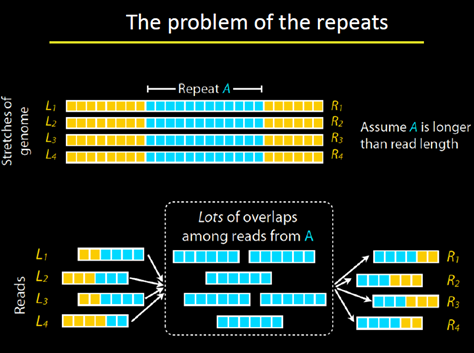
\includegraphics[width=0.6\textwidth]{Repeats.png}
        \caption{Example of genome with repeats}
        \end{figure}

        If the read length is not long at least the length of the repeat a solution cannot be found.
        It will be impossible to determine the length of these repeated regions.
        Also in the graph there will be a lot of cycles and connecting the two extreme of the repeat will not be possible.
        With overlaps graph in particular repeats can cause the production of wrong contigs that assume that two region are sequential when they are not.
        Hints of the presence of repeats are:

        \begin{multicols}{2}
            \begin{itemize}
                \item Region with an abnormally higher coverage.
                \item Pairs over repeated regions have a shorter insert size.
            \end{itemize}
        \end{multicols}

            \paragraph{Solve trough coverage}
            This problem can be partially solved through coverage: assuming that the repeat has the same coverage of all other reads an expected length of the region could be computed.
            This is risky because repeated regions are problematic for the sequencers and a change in coverage for these region could happen.

            \paragraph{Stopping the contig}
            Stopping the contig before the repetitive region and starting it after it is the safest solution.

            \paragraph{Long reads}
            Sequencing with reads longer than the repeat is the only true solution.

\subsection{Solving an overlap graph}
The ideal way to solve the overlap graph is to find all Hamiltonian paths.
These paths connect all nodes once and they provide all possible solutions.
The best path is the one that maximizes the score of the overlaps.
This problem however is NP-hard and not feasible.
Another approach is to use a greedy approach:

\begin{multicols}{2}
    \begin{enumerate}
        \item Randomly select a starting node.
        \item Select the connected node with maximum overlap as the next visitor.
    \end{enumerate}
\end{multicols}

This approach will find a local optimal solution which could not be the global optimum.

\subsubsection{Graph simplification operations}
To minimize the number of operation needed to solve the overlapping graph some simplification operations are needed.
These can be:

\begin{multicols}{2}
    \begin{itemize}
        \item Merging consecutive nodes: if among more reads there is only one possible path they can be merged without loosing any information.
            Nodes that are sequentially connected only with each other are linked together.
        \item  Remove dead ends: if some reads are branching from a path toward a dead-end, they can be removed.
            The removed path could be the right one and some information is lost.
    \end{itemize}
\end{multicols}

\subsubsection{Limitation of overlap graphs}
Overlap graphs have some limitations:

\begin{itemize}
    \item they are problematic when dealing with repeats: maximizing the overall weight will produce wrong assemblies.
    \item They are not tractable: finding the optimal solution is not computationally feasible.
\end{itemize}

Overlap graphs can work to some extent, but now other algorithms are used in assemblers, like the de Bruijn Graphs (DBG) and the Overlap Layout Consensus (OLC).

\begin{figure}[h]
\centering
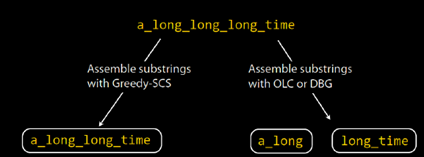
\includegraphics[width=0.6\textwidth]{DBG.png}
\caption{}
\end{figure}

In the case of DBG for example, when facing repeats the contig is split into two: better two right contig than one wrong contig.

\subsection{De Brujin graph assembly}
In De Brujin graph assembly a graph is build such that:

\begin{multicols}{2}
    \begin{itemize}
        \item Nodes are all the unique $k$-mers present in the input reads.
            Where $k$ is an hyperparameter chosen such that it is smaller than the reads lengths.
        \item Edges are the overlaps of the k-mers of length $k+1$ from $2$ sequences.
    \end{itemize}
\end{multicols}

The objective is to find the Eulerian path in the graph (path in which all edges are visited exactly once).
This search is much more efficient than the one of the Hamiltonian path.
Moreover the set of notes will not be too big compared with the number of reads.
When choosing $k$ a trade-off between number of nodes and edges needs to be done.
The $k$-mers that appears only once with great coverage can be removed as they are result of sequencing error, pruning in this way the graph.
Within the graph the paths are more linear with less possibility for wrong cycles to appear.


\section{Post-assembly operations}

    \subsection{Scaffolding}
    Scaffolding is an operation that tries to link together two contigs into a scaffold, consisting of sequences separated by gaps of known length.
    This can be done with paired-end sequencing or estimation of coverage.

    \subsection{Evaluating assemblies}
    N50 length is the sequence length of the shortest contig such that $50\%$ of the sequence is contained in in it.
    Increasing the length of contigs increases in turn the N50, which can be used as a measure of the quality of the assembly process.
